\documentclass[usenames,dvipsnames]{beamer}

\usepackage{acronym}
\usepackage[backend=bibtex]{biblatex}
\usepackage{default}
\usepackage{graphicx}
\usepackage[utf8]{inputenc}
\usepackage{listings}
\usepackage{lmodern}
\usepackage{nameref}
\usepackage{textcomp}

\graphicspath{{figures/}}
\acrodef{BST}{Binary Search Tree}
\acrodef{CAS}{Compare-And-Swap}
\acrodef{CBPQ}{Chunk-Based Priority Queue}
\acrodef{DCAS}{Double-Compare-And-Swap}
\acrodef{DCSS}{Double-Compare-Single-Swap}
\acrodef{DLSM}{Distributed LSM}
\acrodef{DS}{Data Structure}
\acrodef{FAA}{Fetch-And-Add}
\acrodef{FAO}{Fetch-And-Or}
\acrodef{FIFO}{First In First Out}
\acrodef{GSL}{GNU Scientific Library}
\acrodef{LIFO}{Last In First Out}
\acrodef{LSM}{Log-structured Merge Tree}
\acrodef{MOps}{million operations}
\acrodef{NUMA}{non-uniform memory access}
\acrodef{PQ}{Priority Queue}
\acrodef{pthreads}{POSIX Threads}
\acrodef{RAM}{Random Access Memory}
\acrodef{SL}{SkipList}
\acrodef{SLSM}{Shared LSM}
\acrodef{STL}{Standard Library}
\acrodef{TAS}{Test-And-Set}

\bibliography{bibliography.bib}

\setbeamertemplate{bibliography item}{}

\lstset{
    language=C++,
    basicstyle=\ttfamily,
    keywordstyle=\color{OliveGreen},
    commentstyle=\color{Gray},
    captionpos=b,
    breaklines=true,
    breakatwhitespace=false,
    showspaces=false,
    showtabs=false,
    numbers=none,
}

\title{Concurrent Priority Queues}
\subtitle{Seminar in Algorithms, 2013W}
\author{Jakob Gruber, 0203440}
\date{\today}

\usepackage{Sweave}
\begin{document}

\maketitle

% --------------------------------------------------------------------------------------------------
\section{Introduction} \label{sec:intro}
% --------------------------------------------------------------------------------------------------

\begin{frame}[fragile,allowframebreaks]{\nameref{sec:intro}}
\acp{PQ}:

\begin{itemize}
\item Standard abstract data structure
\item Used widely in algorithmics, operating systems, task scheduling, etc
\item Interface consists of two $O(\log n)$ operations:

\begin{lstlisting}
void Insert(pq_t *pq, key_t k, value_t v)
bool DeleteMin(pq_t *pq, value_t *v)
\end{lstlisting}

\item Typical backing data structures: heaps \& search trees
\end{itemize}

\framebreak

\begin{itemize}
\item In the past decade, processor clock speeds have remained the same, trend towards multiple cores
\item New data structures required to take advantage of concurrent execution
\item The topic of this presentation: efficient concurrent \acp{PQ}
\item Fine-grained locking \textrightarrow ~ Lock-free \textrightarrow ~ Relaxed data structures
\end{itemize}

\end{frame}

\begin{frame}{Concepts and Definitions}
\framesubtitle{Safety conditions: nothing bad has happened yet}

\begin{itemize}
\item \emph{Linearizability}: operations appear to take effect at a single point in time, the linearization point
\item \emph{Quiescent consistency}: in a period of quiescence, semantics equivalent to some sequential ordering
\end{itemize}
\end{frame}

\begin{frame}{Concepts and Definitions}
\framesubtitle{Liveness conditions: something good eventually happens}

\begin{itemize}
\item \emph{Lock-freedom}: at least a single process makes progress at all times
\item \emph{Wait-freedom}: every process finishes in a bounded number of steps
\end{itemize}
\end{frame}

\begin{frame}[fragile]{Concepts and Definitions}
\framesubtitle{Miscellaneous}

\begin{itemize}
\item \emph{Disjoint-access parallelism}: how well a data structure handles concurrent use by multiple
      threads within disjoint areas
\item Synchronization primitives:
    \begin{itemize}
    \item \ac{CAS}, \ac{FAA}, \ac{FAO}, \ac{TAS}
    \item \ac{DCAS}, \ac{DCSS}
    \end{itemize}
\end{itemize}

\begin{lstlisting}
bool CAS(T *ptr, T *expected, T value) {
  if (*ptr == *expected) {
    *ptr = value;
    return true;
  } else {
    *expected = *ptr;
    return false;
  }
}
\end{lstlisting}
\end{frame}

% --------------------------------------------------------------------------------------------------
\section{Related Work} \label{sec:related}
% --------------------------------------------------------------------------------------------------

\begin{frame}{\nameref{sec:related}}
\begin{itemize}
\item Non-standard synchronization primitives
    \begin{itemize}
    \item \citeauthor{liu2012lock}: Array-based \ac{PQ} with \lstinline|ExtractMany|
    \item \citeauthor{israeli1993efficient}: Wait-free \ac{PQ}
    \end{itemize}

\item Bounded range priorities
    \begin{itemize}
    \item \citeauthor{shavit1999scalable}: Combining funnels \& bins
    \end{itemize}

\item Strict \acp{PQ}
    \begin{itemize}
    \item \citeauthor{hunt1996efficient}: \textcolor{BrickRed}{Fine-grained locking heap}
    \item \citeauthor{shavit2000skiplist}: \textcolor{BrickRed}{First SkipList-based \ac{PQ}}
    \item \citeauthor{sundell2003fast}: \textcolor{BrickRed}{First lock-free \ac{PQ}}
    \item \citeauthor{linden2013skiplist}: \textcolor{BrickRed}{Minimizes contention}
    \end{itemize}

\item Relaxed data structures
    \begin{itemize}
    \item \citeauthor{kirsch2012fast}: k-FIFO queues
    \item \citeauthor{wimmer2013data}: \textcolor{BrickRed}{k-\ac{PQ}}
    \item \citeauthor{alistarhspraylist}: \textcolor{BrickRed}{SprayList}
    \end{itemize}

\let\thefootnote\relax\footnote{Highlighted \acp{PQ} are presented in the following}

\end{itemize}
\end{frame}

% --------------------------------------------------------------------------------------------------
\section{Fine-grained Locking Heaps} \label{sec:locking}
% --------------------------------------------------------------------------------------------------

% TODO: Figure? Whiteboard demo? 1 summary slide only?

\begin{frame}{\nameref{sec:locking}}
\framesubtitle{\citeauthor{hunt1996efficient}}

\begin{itemize}
\item Naive \ac{PQ} parallelization: single global lock \textrightarrow ~ sequential bottleneck
\item A first improvement: fine-grained locking using a lock per node
\item \fullcite{hunt1996efficient}
\end{itemize}
\end{frame}

\begin{frame}{\nameref{sec:locking}}
\framesubtitle{\citeauthor{hunt1996efficient}: Innovations}

\begin{itemize}
\item One lock per node, \emph{but} additionally a global lock protecting the heap's
      \lstinline|size| variable
\item Insertions bottom-up, deletions top-down to reduce contention
\item Successive insertions take disjoint paths towards the root
\end{itemize}
\end{frame}

\begin{frame}{\nameref{sec:locking}}
\framesubtitle{\citeauthor{hunt1996efficient}: Limitations}

\begin{itemize}
\item A global lock remains
\item Heap is statically allocated
\item Frequent complex heap reorganization
\item Disjoint-access breaks down at high traffic levels
\item Inherent \ac{PQ} bottleneck at the minimal node
\item Benchmarks show only limited scalability up to a low thread count
\end{itemize}
\end{frame}

% --------------------------------------------------------------------------------------------------
\section{Lock-free Priority Queues} \label{sec:lockfree}
% --------------------------------------------------------------------------------------------------

\begin{frame}{\nameref{sec:lockfree}}
\framesubtitle{SkipLists}

\begin{itemize}
\item Modern concurrent \acp{PQ} are mostly based on \citeauthor{pugh1990skip}'s \ac{SL}
\item Probabilistic ordered search structure, insertions and deletions in expected $O(\log n)$ time
\item No reorganizations
\item Simple implementation
\item Excellent disjoint-access properties
\end{itemize}
\end{frame}

\begin{frame}[fragile]{\nameref{sec:lockfree}}
\framesubtitle{SkipLists}

\begin{itemize}
\item Collection of linked lists with corresponding levels
\item Lowest list contains all items, higher lists are shortcuts
\item \lstinline|Insert| chooses a \lstinline|level| according to geometric distribution
\end{itemize}

\begin{lstlisting}
struct slist_t {
  size_t max_level;
  node_t head[max_level];
};
struct node_t {
  key_t key;
  value_t value;
  size_t level;
  node_t *next[level];
};
\end{lstlisting}
\end{frame}


\begin{frame}{\nameref{sec:lockfree}}
\framesubtitle{\citeauthor{shavit2000skiplist}}

\begin{itemize}
\item First SkipList-based \ac{PQ}
\item \fullcite{shavit2000skiplist}
\item Initially lock-based (linearizable), lock-free (quiescently consistent)
      variant published in 2008
\item \fullcite{herlihy2012art}
\end{itemize}
\end{frame}

\begin{frame}{\nameref{sec:lockfree}}
\framesubtitle{\citeauthor{shavit2000skiplist}}

\begin{figure}
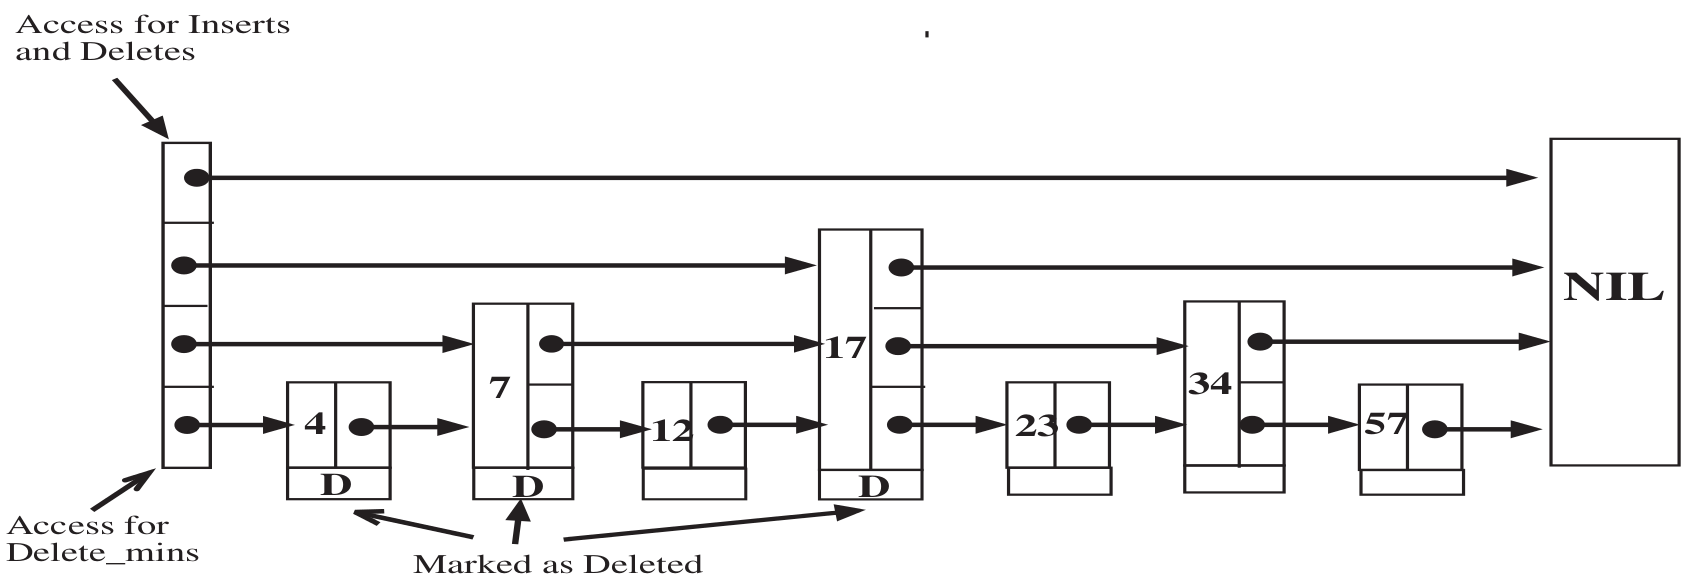
\includegraphics[width=\textwidth]{shavit_lotan}
\caption{The \citeauthor{shavit2000skiplist} \ac{PQ} (Image source: \cite{shavit2000skiplist})}
\end{figure}
\end{frame}

\begin{frame}{\nameref{sec:lockfree}}
\framesubtitle{\citeauthor{shavit2000skiplist}}

\begin{itemize}
\item Items are considered in the list once inserted on bottom level
\item Again, insertions bottom-up and deletions top-down
\item Deletions are split
    \begin{itemize}
    \item Logical deletion sets a \lstinline|deleted| flag
    \item Physical deletion performs actual pointer manipulations
    \end{itemize}
\item \lstinline|DeleteMin| attempts to logically delete the head node.
     On success: delete physically \& return node. Otherwise, continue with
     next node.
\item \lstinline|Insert| is equivalent to the \ac{SL} insertion
\end{itemize}
\end{frame}

\begin{frame}{\nameref{sec:lockfree}}
\framesubtitle{\citeauthor{shavit2000skiplist}}

\begin{itemize}
\item Quiescently consistent, but not linearizable
    \begin{itemize}
    \item Slow thread A suspended at deleted key $k$ while in \lstinline|DeleteMin|
    \item Fast thread B first inserts $k-1$, then $k+1$
    \item A wakes up and returns $k+1$
    \item Linearizability would require returning $k-1$
    \end{itemize}

\item Timestamp mechanism: stamp nodes on successful insertion,
      \lstinline|DeleteMin| ignores all stamps earlier than its own starting point
\item Improved scalability, but heavy contention at list head
\end{itemize}
\end{frame}

\begin{frame}{\nameref{sec:lockfree}}
\framesubtitle{\citeauthor{sundell2003fast}}

\begin{itemize}
\item First lock-free \ac{PQ}, linearizable, \ac{SL}-based, distinct priorities
\item Deletion flag packed into least significant bits of \lstinline|next| pointers
      prevent insertion \emph{after} deleted nodes
\item Helping mechanism ensures only a single logically deleted node exists at any time
\item Performs significantly better than the \citeauthor{hunt1996efficient} heap, slightly better
      than a SkipList protected by a global lock
\item \fullcite{sundell2003fast}
\end{itemize}
\end{frame}

\begin{frame}{\nameref{sec:lockfree}}
\framesubtitle{\citeauthor{linden2013skiplist}}

\begin{itemize}
\item Most efficient strict \ac{PQ}, \ac{SL}-based \& linearizable
\item Concurrent strict \ac{PQ} performance limited by contention and \ac{CAS} failures in
      \lstinline|DeleteMin| \textrightarrow ~ Minimize \ac{CAS} calls
\item Deleted nodes form prefix of \ac{SL}, deletion flag packed into \lstinline|next| pointer of
      \emph{previous} node prevents insertion \emph{before} deleted node
\item Most \lstinline|DeleteMin| perform logical deletion (1 \ac{CAS}) only, physical deletion
      only once a bound is reached
\item Improves upon best previous \acp{PQ} by up to factor 2
\item \fullcite{linden2013skiplist}
\end{itemize}
\end{frame}

\begin{frame}{\nameref{sec:lockfree}}
\framesubtitle{\citeauthor{linden2013skiplist}}

\begin{figure}
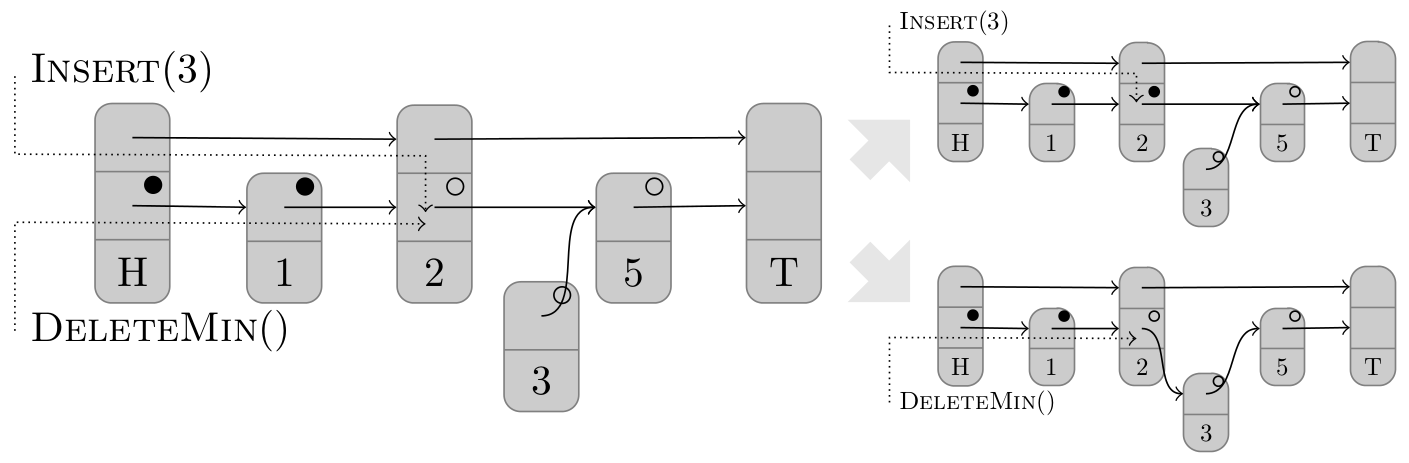
\includegraphics[width=\textwidth]{linden}
\caption{The \citeauthor{linden2013skiplist} \ac{PQ}. Concurrent \lstinline|Insert(3)| and
\lstinline|DeleteMin| operations. Top right: \lstinline|DeleteMin| succeeds first,
\lstinline|Insert(3)| \ac{CAS} fails. Bottom right: \lstinline|Insert(3)| succeeds first,
\lstinline|DeleteMin| returns 3. (Image source: \cite{linden2013skiplist})}
\end{figure}
\end{frame}

% --------------------------------------------------------------------------------------------------
\section{Relaxed Priority Queues} \label{sec:relaxed}
% --------------------------------------------------------------------------------------------------

\begin{frame}{\nameref{sec:relaxed}}

\begin{itemize}
\item Strict \acp{PQ} have inherent bottleneck at minimal element
\item To improve further: $< 1$ \ac{CAS} per \lstinline|DeleteMin|
\item Another approach is to relax semantics, i.e. instead of returning \emph{the} minimal element,
      return one of the $k$ minimal elements
\end{itemize}
\end{frame}

\begin{frame}{\nameref{sec:relaxed}}
\framesubtitle{\citeauthor{alistarhspraylist}}

\begin{itemize}
\item Relaxed \ac{SL}-based \ac{PQ}, safety properties unclear
\item \lstinline|DeleteMin| returns one of the $O(P \log^3 P)$ elements
\item Degrades to random-remove if the \ac{PQ} is small compared to thread count $P$ (for $P = 80$,
      $P \log^3 P \approx 7000$)
\item \lstinline|DeleteMin| performs random walk: starting at the list head on some level $l$,
      repeatedly follow a randomized number of \lstinline|next[l]| pointers, descend a randomized
      number of levels
\item Parameters are chosen s.t. each element within the walk has approximately equal probability
      of being returned
\item Benchmarks show scalability comparable to a random-remove \lstinline|Delete| up to at
      least 80 threads
\item \fullcite{alistarhspraylist}
\end{itemize}
\end{frame}

\begin{frame}{\nameref{sec:relaxed}}
\framesubtitle{\citeauthor{wimmer2013data}}
% Essence: Local list, if necessary push to global
\begin{itemize}
\item First relaxed linearizable \acp{PQ}: we discuss the hybrid k-\ac{PQ} which, provides a bound of
      $kP$ missed elements in \lstinline|DeleteMin|
\item Consists of a list of globally visible elements, and per thread: a local item list, and a local
      \ac{PQ}
\item \lstinline|Insert| accesses only the local structures as long as guarantees are not violated,
      otherwise the global list is updated the the local view is synchronized
\item \lstinline|DeleteMin| pops the local queue if it is non-empty; otherwise spy, i.e. copy
      elements from another thread's local list
\item Very good scalability up to 10 threads, further limited gains with rising thread counts
\item \fullcite{wimmer2013data}
\end{itemize}
\end{frame}

\begin{frame}{\nameref{sec:lockfree}}
\framesubtitle{\citeauthor{wimmer2013data}}

\begin{figure}
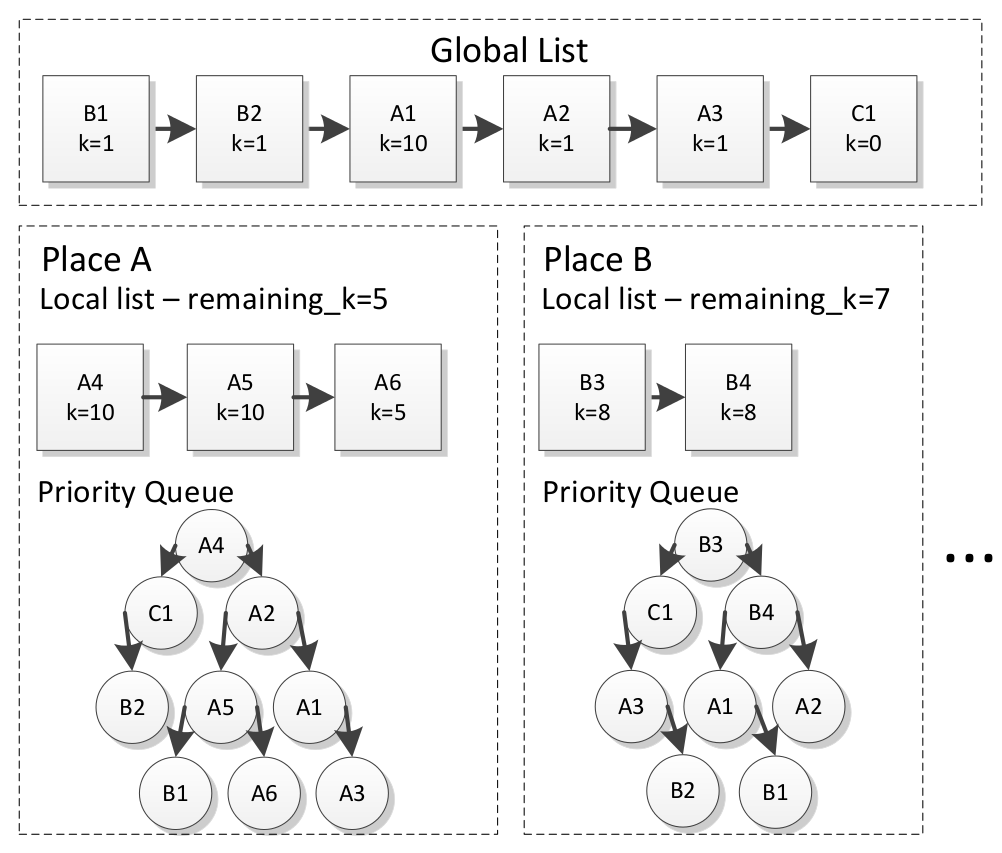
\includegraphics[width = 0.65\textwidth]{wimmer}
\caption{The \citeauthor{wimmer2013data} hybrid k-\ac{PQ}. (Image source: \cite{wimmer2013data})}
\end{figure}
\end{frame}

% --------------------------------------------------------------------------------------------------
\section{Results} \label{sec:Results}
% --------------------------------------------------------------------------------------------------

\begin{frame}{\nameref{sec:Results}}

\begin{itemize}
\item Benchmarking results from selected papers \& own results
\item We present throughput, i.e. the number of operations performed per second
\item Each thread repeatedly chooses uniformly at random between
      \lstinline|Insert| and \lstinline|DeleteMin|
\end{itemize}
\end{frame}

\begin{frame}{\nameref{sec:Results}}
\framesubtitle{\citeauthor{linden2013skiplist}}

\begin{figure}
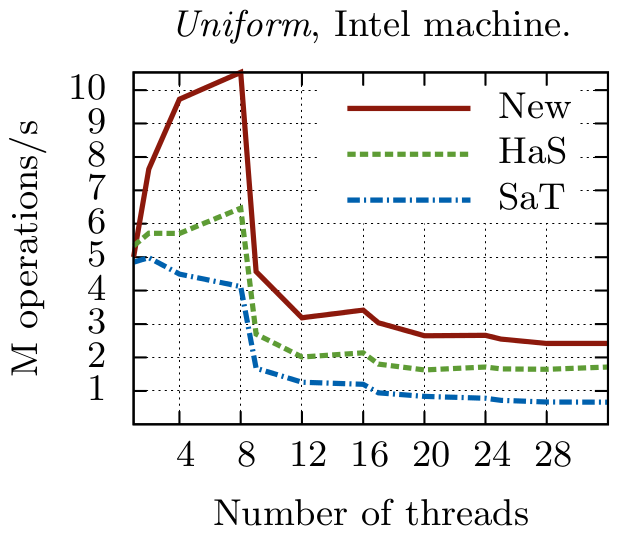
\includegraphics[width=0.6 \textwidth]{results_linden}
\caption{GCC 4.7.2, 32-core Intel Xeon E5-4650 @ 2.7 GHz. Initial \ac{PQ} size unknown.
\emph{New}: \citeauthor{linden2013skiplist},
\emph{HaS}: \citeauthor{shavit2000skiplist},
\emph{SaT}: \citeauthor{sundell2003fast}. 
(Image source: \cite{linden2013skiplist})}
\end{figure}
\end{frame}

\begin{frame}{\nameref{sec:Results}}
\framesubtitle{Gruber}
\end{frame}

\begin{frame}{\nameref{sec:Results}}
\framesubtitle{\citeauthor{alistarhspraylist}}
% 10^6
\begin{figure}
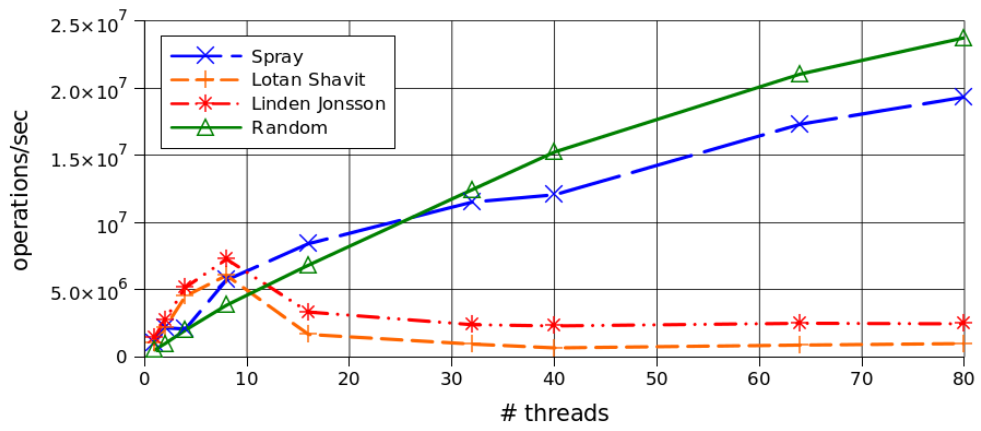
\includegraphics[width=\textwidth]{results_spraylist}
\caption{GCC version unknown, 80-core Intel Xeon E7-4870 @ 2.4 GHz. \ac{PQ} initialized with $10^6$
elements.
(Image source: \cite{alistarhspraylist})}
\end{figure}
\end{frame}

% --------------------------------------------------------------------------------------------------
\section{Conclusion} \label{sec:conclusion}
% --------------------------------------------------------------------------------------------------

\begin{frame}{\nameref{sec:conclusion}}
\begin{itemize}
\item Parallelizing \acp{PQ} is hard
\item SkipLists currently dominate practical implementations
\item Main limiting factor are list head accesses in \lstinline|DeleteMin|
\item \citeauthor{linden2013skiplist} \ac{PQ} is state of the art in strict
      semantics
\item Much potential remains in relaxed \acp{PQ} and data structures in general
      \textrightarrow ~ future research
\end{itemize}
\end{frame}

\begin{frame}{\nameref{sec:conclusion}}
\centering
Questions?
\end{frame}

% --------------------------------------------------------------------------------------------------
\section{References} \label{sec:references}
% --------------------------------------------------------------------------------------------------

\begin{frame}[allowframebreaks]{\nameref{sec:references}}
\printbibliography
\end{frame}

\end{document}
